\documentclass{article}
\usepackage[utf8]{inputenc}
\usepackage{polski}
\usepackage{hyperref}
\usepackage{listings}
\usepackage{mathtools}
\usepackage{graphicx}
\usepackage[]{algorithm2e}
\usepackage{fullpage}
\usepackage{float}
\usepackage{caption}
\usepackage{subcaption}
\usepackage[parfill]{parskip}
\title{Systemy Uczące Się \\ Grupowanie/Klasteryzacja}
\author{Michał Zając \\ 203229}
\graphicspath{ {images/} }
\date{16 grudnia 2016}
\begin{document}
\maketitle
\clearpage
\section{Wstęp}
Zapoznanie się z systemem R wspierającym statystyczne obliczenia i metody uczenia maszynowego, na przykładzie zagadnienia klasteryzacji (czasem zwaną grupowaniem) danych.

\section{Algorytm K-means}
 
Algorytm K-means jest heurystyczną metodą wyznaczania klastrów, do których przydzielane są wszystkie elementy zbioru. Przebieg algorytmu wygląda następująco:
 
\begin{enumerate}
\item Wybieramy \emph{k} losowych punktów jako centroidy.
\item Każdy element zbioru obserwacji przypisujemy do najbliższego centroidu na podstawie odległości euklidesowej.
\item Obliczamy nowy centroid bazując na średniej wartości poszczególnych atrybutów w centroidzie.
\item Kroki 2-3 powtarzamy dopóki nie nastąpi modyfikacja pomiędzy krokami, lub nie zostanie spełniony inny warunek stopu.
\end{enumerate}
 
\section{Algorytm PAM}
 
W algorytmie PAM zamiast centroidów środek klastra(zwanych tutaj medoidami) zawsze jest jednym z obiektów, który znajduje się w zbiorze. Właściwy algorytm prezentuje się następująco:
 
\begin{enumerate}
\item Wybieramy \emph{k} losowych punktów jako medoidy.
\item Każdy element zbioru obserwacji przypisujemy do najbliższego centroidu na podstawie odległości euklidesowej.
\item Dopóki odległość między punktami zmniejsza się:
\begin{enumerate}
\item Dla każdego medoida i każdego obiektu nie będącego medoidem zamień je funkcjami (uznaj medoid za zwykły obiekt a wybrany obiekt za medoid). Jeżeli odległość się zwiększy od poprzedniego kroku, cofnij zmianę.
\item Każdy obiekt z klastra potraktuj jako medoid. Jeżeli odległość między obiektami nie zmniejszy się w stosunku do poprzedniego kroku to cofnij zmianę.
\end{enumerate}
\end{enumerate}

\section{Wybrane zbiory danych}
Do ćwiczenia użyto następujących zbiorów danych:
\begin{description}
\item[Iris] -  zbiór danych o irysach. Występują w nim trzy możliwe klasyfikacje, w zależności od gatunku kwiatu. Liczba cech: 4. Liczebność zbioru: 150
\item[Pima Indians Diabetes] - zbiór zawierający dane o osobach z USA, którzy chorują na cukrzycę. Występują w nim dwie możliwe klasyfikacje: osoba chora i osoba zdrowa. Liczba cech: 8. Liczebność zbioru: 768
\item[Ionosphere] - zbiór danych zawiera dane dotyczące jonosfery zebrane z 16 anten. Dwie klasy, liczba cech: 34, liczebność zbioru: 351.
\end{description}

\section{Implementacja}
Do wykonania zadania napisano skrypt w języku R wykonujący potrzebne obliczenia.

\section{K-means}
\subsection{Iris}
\subsubsection{3-fold crossvalidation}
\begin{figure}[p]
    \centering
    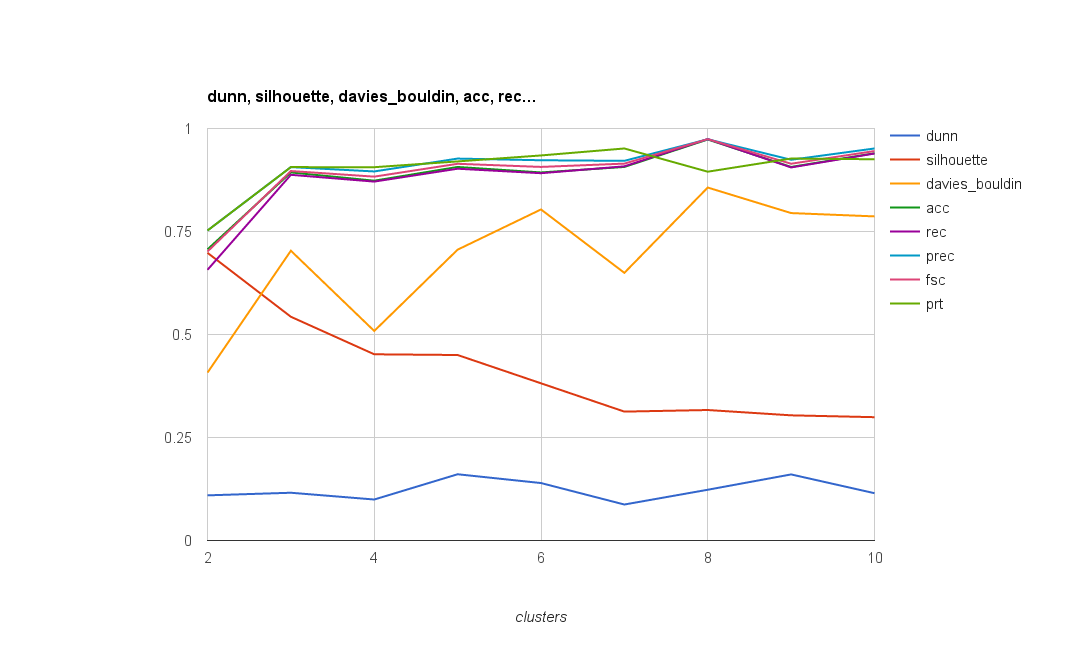
\includegraphics[width=0.8\textwidth]{kmeans_iris.arff_3}
\end{figure}
\subsubsection{5-fold crossvalidation}
\begin{figure}[p]
    \centering
    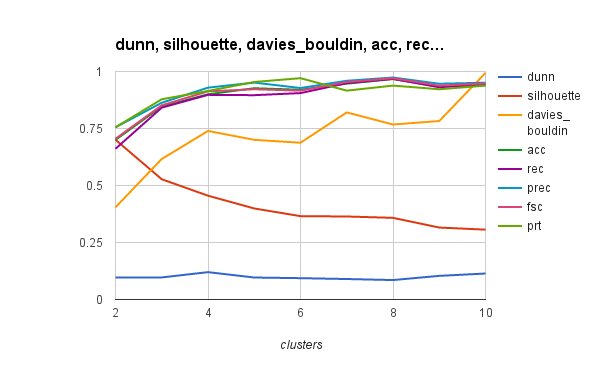
\includegraphics[width=0.8\textwidth]{kmeans_iris.arff_5}
\end{figure}
\subsubsection{10-fold crossvalidation}
\begin{figure}[p]
    \centering
    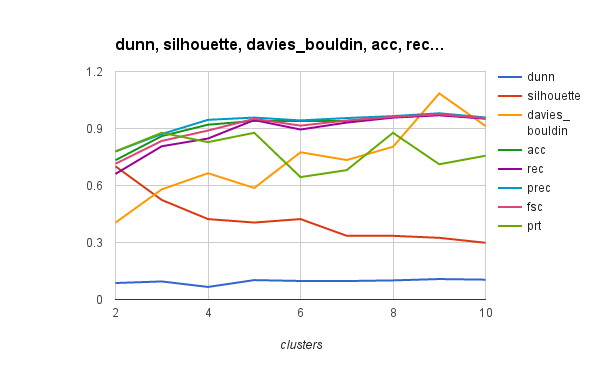
\includegraphics[width=0.8\textwidth]{kmeans_iris.arff_10}
\end{figure}
\subsection{Diabetes}
\subsubsection{3-fold crossvalidation}
\begin{figure}[p]
    \centering
    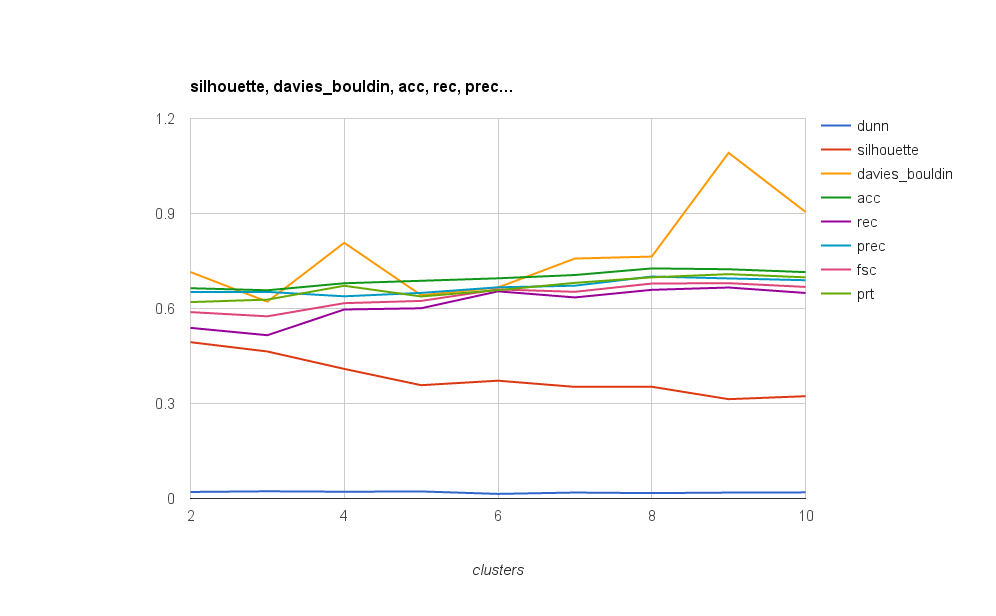
\includegraphics[width=0.8\textwidth]{kmeans_diabetes.arff_3}
\end{figure}
\subsubsection{5-fold crossvalidation}
\begin{figure}[p]
    \centering
    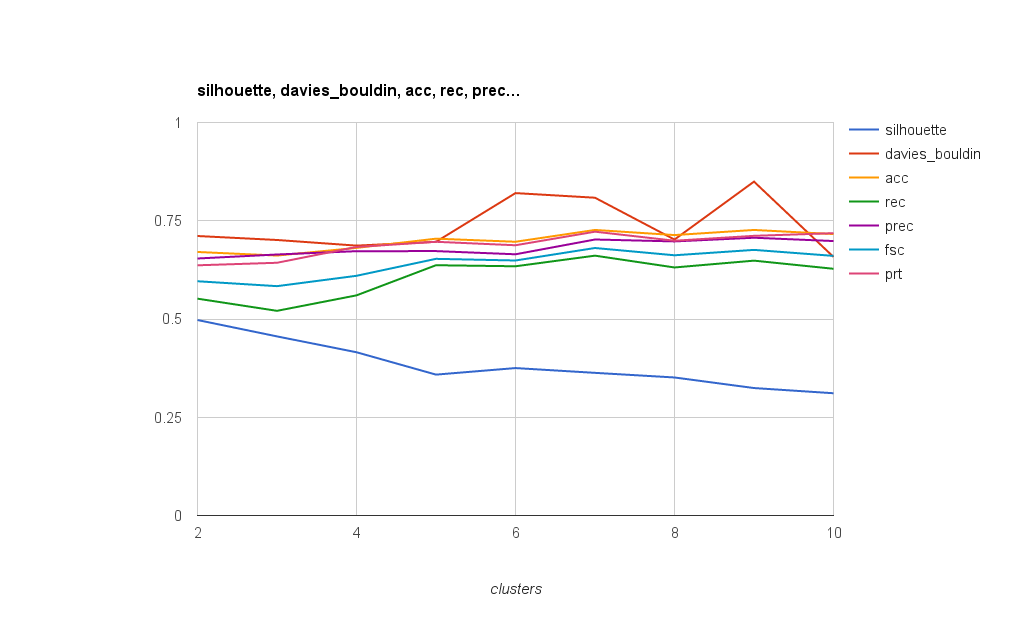
\includegraphics[width=0.8\textwidth]{kmeans_diabetes.arff_5}
\end{figure}
\subsubsection{10-fold crossvalidation}
\begin{figure}[p]
    \centering
    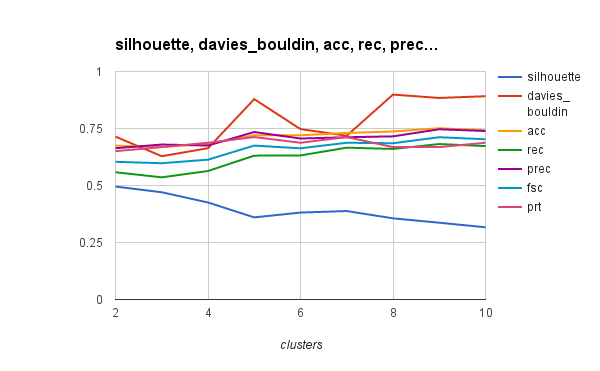
\includegraphics[width=0.8\textwidth]{kmeans_diabetes.arff_10}
\end{figure}
\subsection{Ionosphere}
\subsubsection{3-fold crossvalidation}
\begin{figure}[p]
    \centering
    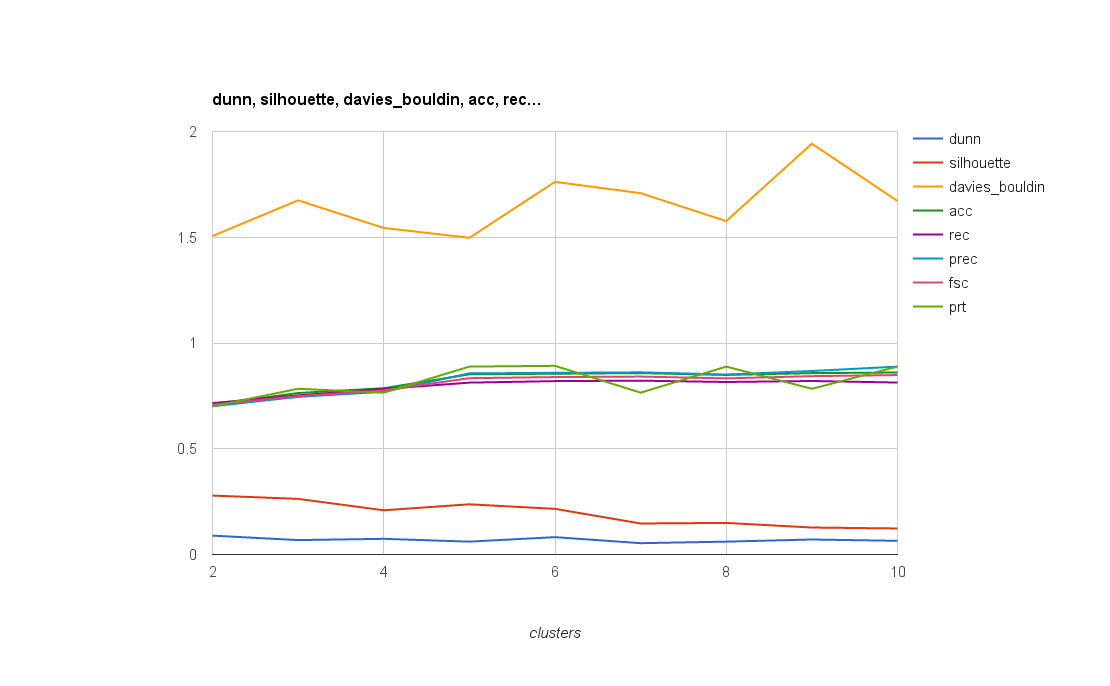
\includegraphics[width=0.8\textwidth]{kmeans_ionosphere.arff_3}
\end{figure}
\subsubsection{5-fold crossvalidation}
\begin{figure}[p]
    \centering
    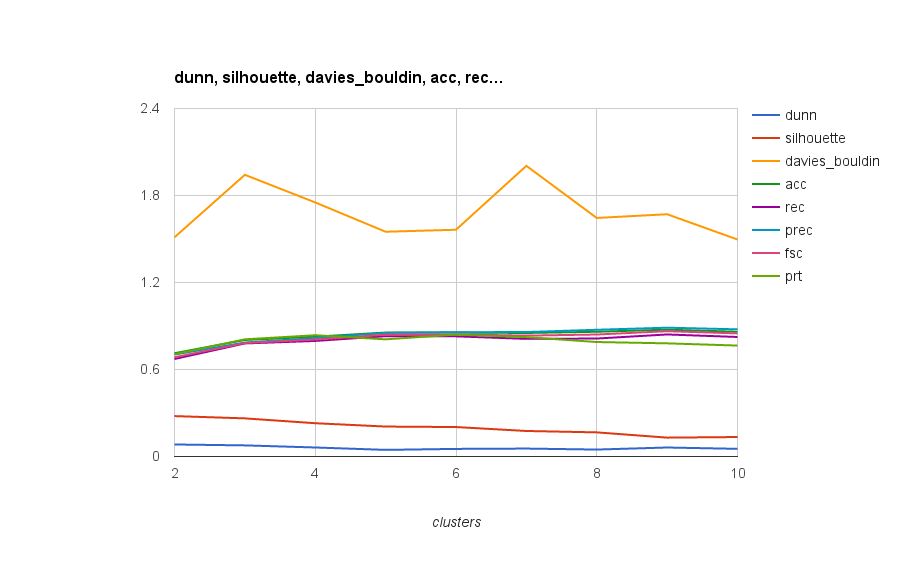
\includegraphics[width=0.8\textwidth]{kmeans_ionosphere.arff_5}
\end{figure}
\subsubsection{10-fold crossvalidation}
\begin{figure}[p]
    \centering
    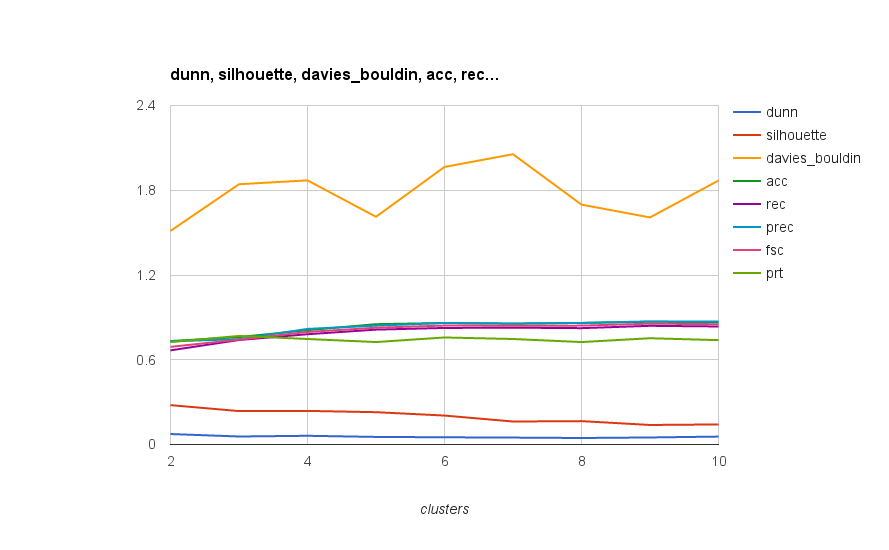
\includegraphics[width=0.8\textwidth]{kmeans_ionosphere.arff_10}
\end{figure}

\section{PAM}
\subsection{Iris}
\subsubsection{3-fold crossvalidation}
\begin{figure}[p]
    \centering
    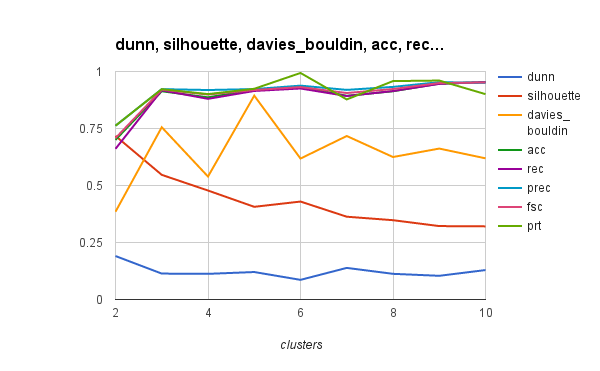
\includegraphics[width=0.8\textwidth]{pam_iris.arff_3}
\end{figure}
\subsubsection{5-fold crossvalidation}
\begin{figure}[p]
    \centering
    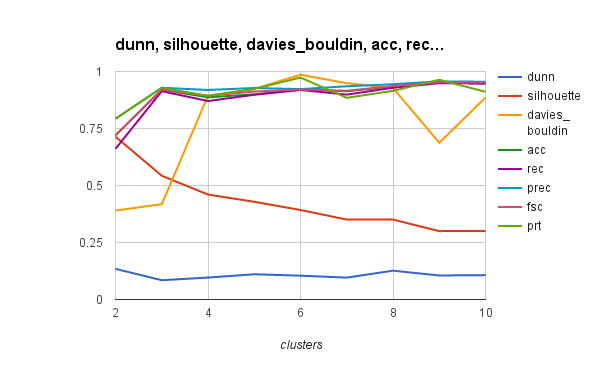
\includegraphics[width=0.8\textwidth]{pam_iris.arff_5}
\end{figure}
\subsubsection{10-fold crossvalidation}
\begin{figure}[p]
    \centering
    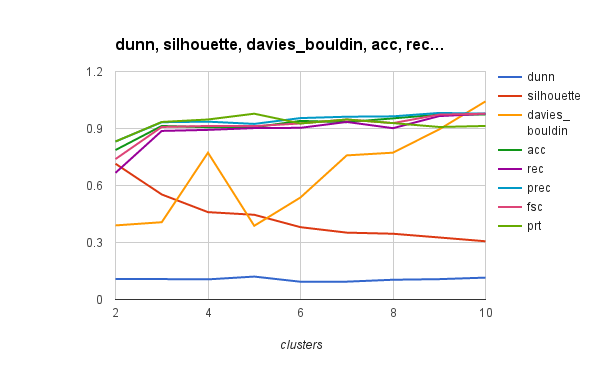
\includegraphics[width=0.8\textwidth]{pam_iris.arff_10}
\end{figure}
\subsection{Diabetes}
\subsubsection{3-fold crossvalidation}
\begin{figure}[p]
    \centering
    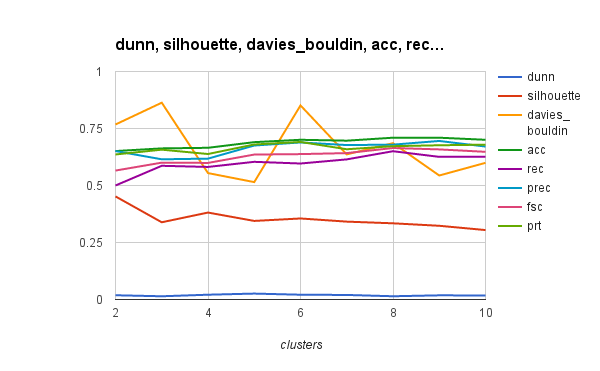
\includegraphics[width=0.8\textwidth]{pam_diabetes.arff_3}
\end{figure}
\subsubsection{5-fold crossvalidation}
\begin{figure}[p]
    \centering
    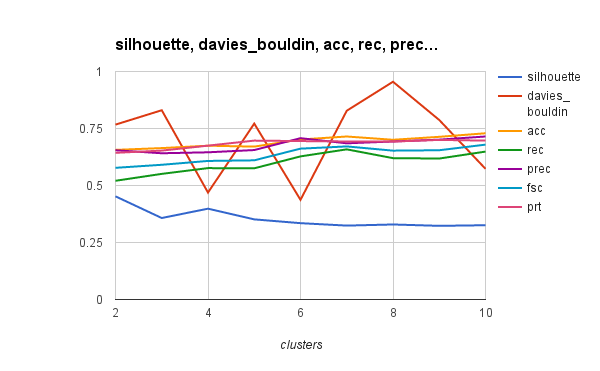
\includegraphics[width=0.8\textwidth]{pam_diabetes.arff_5}
\end{figure}
\subsubsection{10-fold crossvalidation}
\begin{figure}[p]
    \centering
    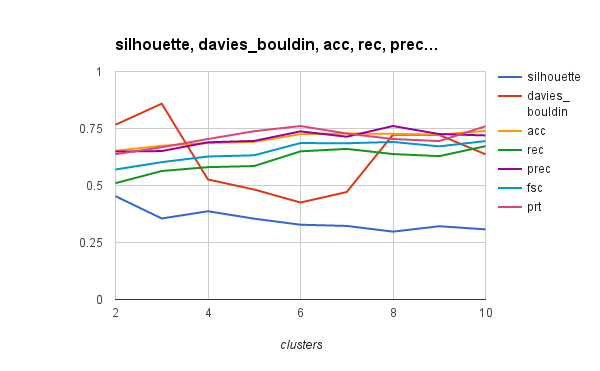
\includegraphics[width=0.8\textwidth]{pam_diabetes.arff_10}
\end{figure}
\subsection{Ionosphere}
\subsubsection{3-fold crossvalidation}
\begin{figure}[p]
    \centering
    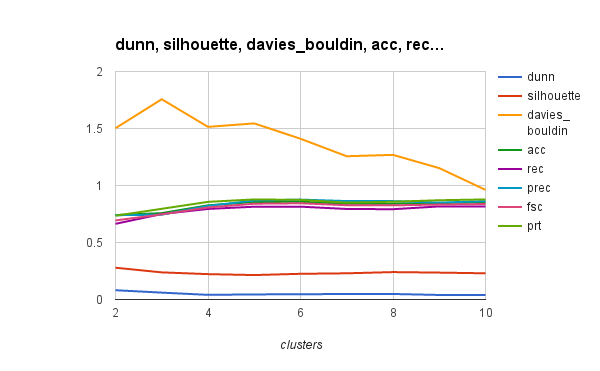
\includegraphics[width=0.8\textwidth]{pam_ionosphere.arff_3}
\end{figure}
\subsubsection{5-fold crossvalidation}
\begin{figure}[p]
    \centering
    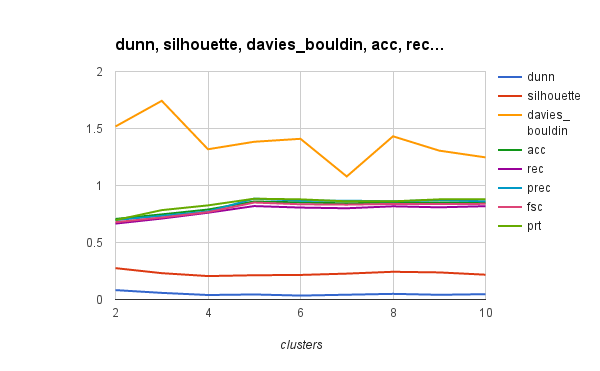
\includegraphics[width=0.8\textwidth]{pam_ionosphere.arff_5}
\end{figure}
\subsubsection{10-fold crossvalidation}
\begin{figure}[p]
    \centering
    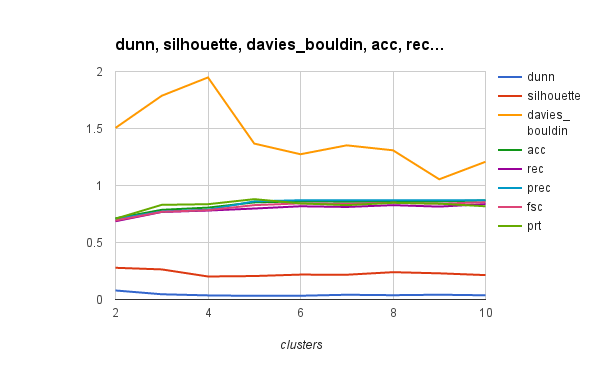
\includegraphics[width=0.8\textwidth]{pam_ionosphere.arff_10}
\end{figure}

\begin{thebibliography}{1} 
\bibitem{zbiory} Lichman, M. (2013). \href{http://archive.ics.uci.edu/ml}{UCI Machine Learning Repository}. Irvine, CA: University of California, School of Information and Computer Science.
\bibitem{parkinsons} \emph{Exploiting Nonlinear Recurrence and Fractal Scaling Properties for Voice Disorder Detection}, Little MA, McSharry PE, Roberts SJ, Costello DAE, Moroz IM. BioMedical Engineering OnLine 2007, 6:23 (26 June 2007)
\bibitem{discret} \href{http://robotics.stanford.edu/users/sahami/papers-dir/disc.pdf}{Supervised and Unsupervised Discretization of Continous Features} - Dougherty, J., Kohavi, R., Sahami, M., Computer Science University, Stanford University 
\bibitem{ila} \href{http://www.dis.uniroma1.it/~sassano/STAGE/LearningRule.pdf}{An Inductive Learning Algorithm for Production Rule Discovery} - Tolun, M.R., Abu-Soud, S.M. 1999
\bibitem{wykladKw} Indukcja reguł, podejście sekwencyjnego pokrywania, algorytm AQ - Systemy Uczące Się. Slajdy do wykładu prof. dr hab. inż. Haliny Kwaśnickiej, Politechnika Wrocławska.
\end{thebibliography}
\end{document}
